\section{Empirical Study/ Testing}


\ref{Fig:VSS}. 
\begin{figure}[ht]
    \begin{center}
        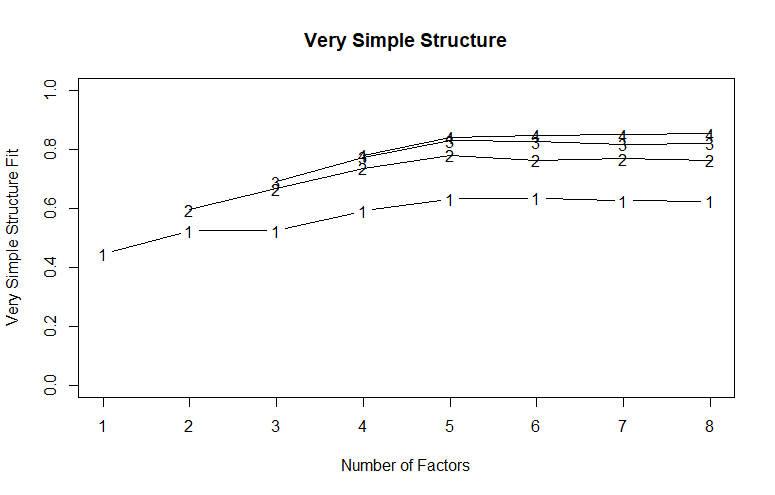
\includegraphics[scale=0.5,angle=0]{Figures/VSS.png}
        \caption{VSS-Analysis}
        \label{Fig:VSS}
    \end{center}
\end{figure}
\newline
The next method is to do a parallel analysis as seen in \ref{Fig:Parallel}.
\begin{figure}[ht]
    \begin{center}
        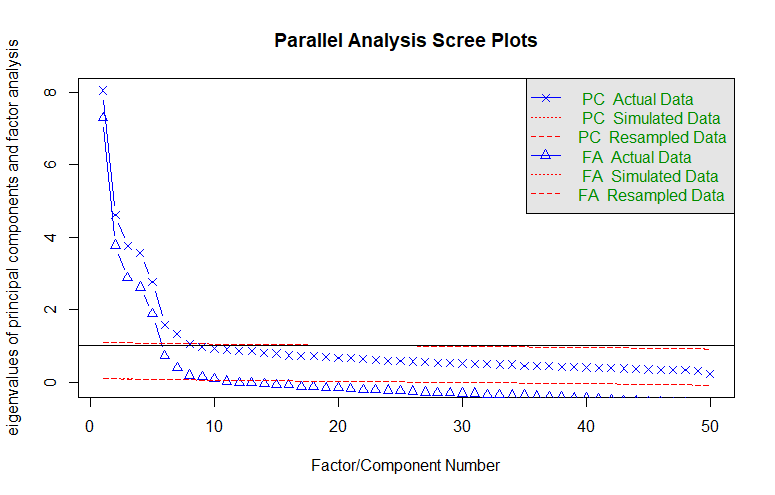
\includegraphics[scale=0.5,angle=0]{Figures/ParallelAnalysis.png}
        \caption{Parallel Analysis}
        \label{Fig:Parallel}
    \end{center}
\end{figure}
\newline

we tested our Data Analysis.R with P-value and T-student  to see whether it is significant or not  and then we compare  the mean of males and the mean of  females  to see which one of gender have thier special personality 

we concluded that in this table :

\begin{table}[ht]
    \begin{center}
        {\footnotesize
        \begin{tabular}{l|l|l|l|l|l|}
        \hline \hline
               & introversion   & neuro    & agree   & openess   & conscient        \\
            \hline
                Mean of males    & -0,06 & -0,22   & -0,27 & -0,054 & 0,14   \\
                Mean of females  & 0,04 & 0,14 & 0,18 & 0,036 & -0,092  \\
                t-student        & 7 & 25 & 31,5 & 6 & 16   \\
                p-value          & 1,213e-12 & 2,2e-16 & 2,2e-16 & 3,373e-10 & 2,2e-16   \\
               
            \hline \hline
        \end{tabular}}
    \end{center}
    
\end{table}

{\normalsize{\bf the results:}} \\\vspace{0.5cm}


we see that the t-student is bigger than T-table wich equal 1,65  with α=0,05     and  Degree of freedom (DF) is bigger than 29
  P-value is smaller than 0,05
and this confirm our rejection hypothesis that mean not equal to zero (or the mean of the females not equal the mean of males) 
  in case Introversion/Extraversion , Neuro, Agree and Openess
we see that the mean of the males is smaller than  the mean of  the females and that mean females are more Introversion/Extraversion,neuro, agree and openness than males
But in case Consient we see that the mean of the males is bigger than  the mean of  the females and that mean males are more consient than females 





TODO: Test your code with an empirical study. Describe the data you use, state the source and how
the data was prepared. Show tests of final code version. Tests may include correct input,
incorrect input, special cases and stress tests etc. Method of testing will vary with the
problem at hand. Present the empirical results of your analysis. Do the results support the
theory? If not, why? \underline{\textbf{This section is very important.}}
\newline
\newline
Display the tests with this format:
\begin{itemize}
  \item Input
  \item Expected output
  \item Actual output
  \item Comments
\end{itemize}


\underline{Data Analysis - Gender Groups:
 \href{https://github.com/Matthias2193/SPL/blob/master/Big5DataAnalysisAgeGender/DataAnalysis_PTGenderAgeGroup.R}{
\includegraphics[scale = 0.06]{Figures/qletlogo.pdf}} :} 
\newline 
\newline
 This file deals with an analysis of all five personality traits (Extraversion, Openness, Conscientiousness, Agreeableness, and Neuroticism) with accordance to the age group. In short, we analysed whether a personality trait changes on average over time. Note, that the analysis from this file was made for a visual interpretation. Among vast academic researches along the topic of personality research, Roberts et al. (2006) have devoted themselves to this specific subject indeed. They found out that an average change in personality traits across the life course appears.
 \newline \newline
 In our study we have tried to show such patterns as well. For that we wanted to receive a visual big picture of the personality traits across the life course with accordance to our data set. 
Our file, in which we applied this study, starts with the general data generation part. With the function source(), we are able to access another file or rather script in order to connect with the already prepared data set which we will need for this study. 
 \newline \newline
When we set up the connection to the main data script, we pulled the data to our script and declared the dataset from the function `getCombinedData(FALSE)' as fiveFactors. We set the last parameter of the function to `FALSE' as we do not want to scale our data output from the test result.
 \newline \newline 
For the next step we created three new data frames in accordance to continue with our study. With the apply function from the package “base” we are able to return a vector of the average personality traits for each age group obtained by applying the mean function on our matrix `fiveFactor' with accordance to their age category. In short we applied a condition in our mean calculation for the personality traits, which is the age category.
\newline \newline
As we already explained, please note that each age category represents 10 years. So, in other words, if the test person is 18 years old it will fall into the age category 2. Further the entry mean, refers to the statistic method to calculate the mean of the entries. The last entry `na.rm=T' simply means that the functions ignores NAs for their calculation.
\newline \newline
The vectors, which the `apply()' functions returned, were called `avgAge[1,9]', where [1,9] refers to each category eg. 1 has been named `avgAge1'.
The generated vectors have been bounded together to a data frame, which was named `ages'.  The function `rbind()' binds all vectors together and with the function “data.frame”, we are able to create a data frame. 
\newline \newline
The same procedure was also applied two more times, however, with an additional condition. The following two data frames, which we created should differ in gender. So, we did the same procedure, but only wanted to take into consideration either male (`fiveDactors\$gender ==1') or female (`fiveDactors\$gender ==2'). The additional condition was added by applying the logical AND `\&'.  
\newline \newline
The generated data frames with respect to the gender group, was defined as `mage' (mean of personality traits with accordance to the age category of the male test persons) and `fage' (same but with respect to only female test persons).
\newline \newline
For the visualisation of our data frames to detect possible changes in personalities across the life course, we continued with plotting the average personality traits with respect to the age group (combined all test persons, only males, and only females).
\newline \newline
In the following we will explain the code by the example of the personality trait `Extraversion'. The following personality traits were applied the exact same procedure, however, intuitively with accordance to the certain personality trait.
\newline \newline
With the function `plot()' we are able to plot our first vector. Our x-axis were assigned to the age categories (ageCat). We only took into consideration group 1-7, due to the fact that age group 8 and 9 showed massive deviation. For comparison, table (XC) will demonstrate it with the example of the personality trait `Extraversion'. The second entry of our `plot()' function referred to the specific personality trait with respect to all test persons (`ages\$Intro'). We selected the line type (our plotted vector should be shown as a line), we specified a colour and we scaled the y-axis for better visualisation. 
\newline \newline
To the generated plot for all test persons, we added two more lines (only males, only females). 
\newline \newline
\begin{figure}[ht]
\setlength{\abovecaptionskip}{-4pt}
\begin{center}
  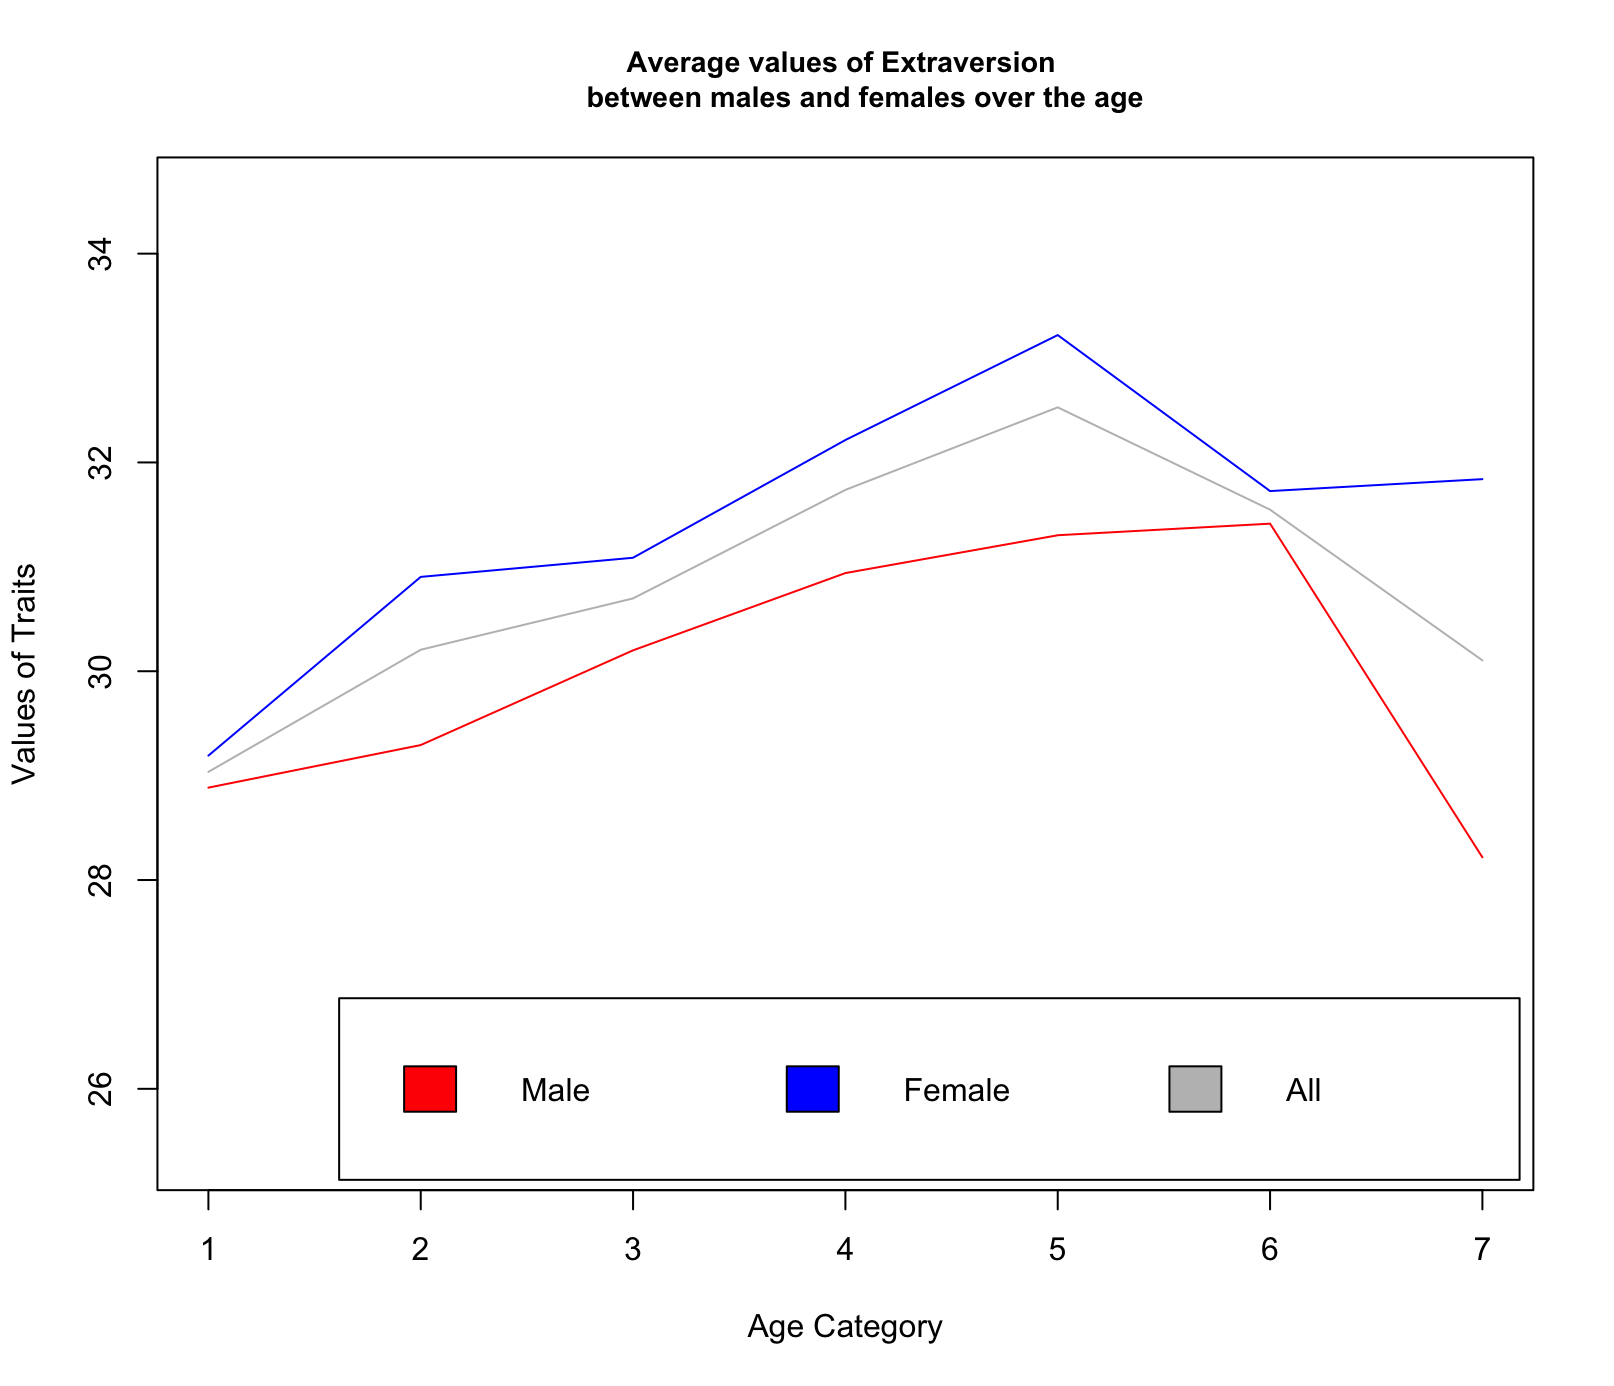
\includegraphics[width=13cm]{Figures/AVG_Extra_Gender}
  \caption{Personality Difference of Age and Gender}
\end{center}
\end{figure}
\newline \newline
With accordance to the figure above, we visually have similar findings as Roberts et al. (2006). Across the life course we have a changing value of trait. In other words, we can conclude that the average score of Extraversion (based on the test result) is increasing by age. However, in age category 5, we see a slightly decresing value for females. For men, we find that the personality (`Extraversion') is decreasing up from age group 6. 
\newline \newline
We have similar findings for our other personality traits. With accordance to our personality test data, we can visually conclude that across the life course we have a changing value. These findings are similar to these in Roberts et al. (2006).
\newline \newline
\underline{Data Analysis - Variance Analysis:
 \href{https://github.com/Matthias2193/SPL/tree/master/Big5VarianceAnalysis}{
\includegraphics[scale = 0.06]{Figures/qletlogo.pdf}} :} 
\newline 
\newline
Further with our study, in file `Variance Analysis – Big 5' we analysed the relationship between personality traits and age. As we have seen it visually that across the life course we have a changing value, we want to calculate that once working with regression models for our personality traits the additional variable age will significantly decrease the variance or rather the fit of the regression. The paper by Srivastava et al. (2003) studied whether the personality changes during adulthood. 
\newline \newline
Therefore, we tested our hypothesis from our visual results that age has an influence on the character over the course of life. 
\newline \newline
For that, we first applied an analysis of variance (ANOVA) in R. With the function `aov()' we were able to perform an ANOVA. We did our study first with the application whether the age of our test persons having a significant impact on the personality trait `Agreeableness'. Our ANOVA showed that the additional variable age improved the fit significantly (on all conventional significant levels). 
\newline \newline
Further, we created ANOVAs for all personality traits against the independent variable for age, hand, race and gender. Are these variables improving the fit and provide additional information?
\newline \newline
We created a function named \href{https://github.com/Matthias2193/SPL/blob/40438376a983799102d15acb98bdd9a0a98a6889/Big5VarianceAnalysis/VarianceAnalysis.R#L13-L26}{
\includegraphics[scale = 0.06]{Figures/qletlogo.pdf}anova\underline{ }multi} to solve this problem in accordance to receive a matrix with all our test results.
\newline \newline
The function first creates an empty matrix with the number of rows in accordance to the personality traits (we have 5) plus the number of columns in accordance to our independent variables (we have 4). The function `names()' calls the row names out of our dataset `DATA', in accordance to name the matrix with their row names. The column names were chosen based on the independent variable. We created a list for that: `c('Test Stat - Gender', 'Test Stat - Age', 'Test Stat - Hand', 'Test Stat - Race')'.
\newline \newline
With the for function we can calculate all the ANOVAs in an iterative way. It calculates for each column 5 times an ANOVA with the different personality traits, but the same independent variable. Once it’s done it will return the matrix in the console. 
\newline \newline
With this function, we are now able to create a matrix of the different p-values out of the F-statistic whether the independent variable increases the variance. A p-value smaller than 0.05 rejects the H0 (on a 5 \% significance level) that the independent variable does not increase fit of the regression. In other words, we want a rejection to conclude that the independent variable decreases the variance and therefore includes further information.
\newline \newline
With the function `anova\underline{ }multi(DATA,DATA{[,2]},DATA{[,3]},DATA{[,4]},DATA{[,5]})' we ran the function on our data set in accordance to the selected independent variables (gender, age, hand, race). 
\newline \newline
With respect to the table above, we can confirm that the personality changes across the course of life.
However, the independent variable `race' does not improve the fit for the personality Extraversion and Neuroticism. In other words, the variance for the regression, when considering “race” as an additional variable, does not decrease for these two. Conscientiousness is only decreasing the variance on a 10\% significant level. Overall, we can conclude that the ANOVA test is overall an important measurement for explaining the fact of personality traits with accordance to independent variables, in particular gender, age, hand, and race. When looking at the independent variables fundamentally, we support the fact for age as we refer to Srivastava et al. (2003). However, the other findings could overall not have a significant impact on explaining the personality traits. 


